\section{Architektur und Komponenten}\label{sec:architektur-und-komponenten}

\begin{itemize}
    \item Diagramm zur Architektur erstellen
    \item HTTP-Endpunkt oder CLI zum Starten -> Holen der notwendigen Testdatensätze -> Aufruf der Klassifizierung pro Modell und pro Testcase -> Akkumulieren der Ergebnisse pro Testcase + ggf. frühzeitige Rückgabe des Ergebnisses des Testcase für Live-Ansicht in UI -> Aufarbeiten der akkumulierten Ergebnisse und berechnen wichtiger Metriken
    \item EvaluationController, MultiEvaluationRunner, EvaluationRunner, HttpEvaluator, MetricsAccumulator, ggf. Frontend (Concurrency von MultiEvaluationRunner)
\end{itemize}

\begin{figure}
    \centering
    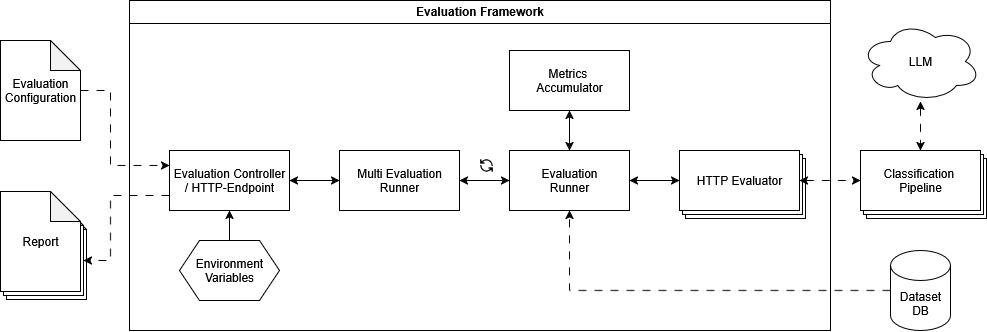
\includegraphics[width=.9\linewidth]{images/evaluation/evaluation-framework-architecture}
    \caption{Architektur des Evaluationsframeworks}
    \label{fig:evaluation-framework-architecture}
\end{figure}